% !TEX encoding = UTF-8
% !TEX TS-program = pdflatex
% !TEX root = ../tesi.tex

\newgeometry{a4paper, left=30mm, right=30mm, top=5mm, bottom=30mm}
%**************************************************************
\chapter{Progettazione e codifica}
\label{cap:progettazione-codifica}
%**************************************************************

\noindent \intro{In questo capitolo vengono esposte le attività di progettazione e codifica del modulo di ottimizzazione.}\\

%**************************************************************
\section{Architettura}
\label{sec:progettazione}
\noindent Prima di descrivere più in particolare l'algoritmo, è necessario
fornire un’idea dell’architettura sulla quale si basa l'intero progetto.
Di seguito è presentato uno schema ad alto livello di come sono strutturate le varie
componenti che formano il sistema.

\begin{figure}[!h] 
    \centering 
    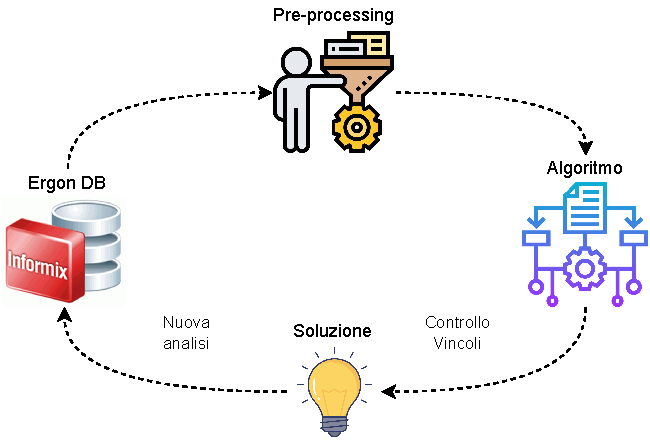
\includegraphics[width=0.95\columnwidth]{architettura/architettura.pdf} 
    \caption{Architettura generale}
    \label{architettura-generale}
\end{figure}

\noindent Come si può notare in figura \ref{architettura-generale},
il flusso del sistema è circolare.
Si parte dal database, dal quale vengono estratti i dati di interesse dalle varie
tabelle. Successivamente viene fatto il pre-processing dei dati,
in modo tale da poter poi eseguire l'ottimizzazione solo su
ciò che è di interesse dell'analisi.
Di seguito viene effettuato il controllo dei vincoli di minimo al termine
dell'algoritmo così da generare
una soluzione ammissibile. Se si vuole effettuare una nuova
analisi è necessario estrarre nuovamente i dati dal
database ed eseguire nuovamente il ciclo. Questo è necessario
in quanto i dati all'interno del database possono variare
(esempio: prezzi, date di spedizione...).

\newpage

\newgeometry{a4paper, left=30mm, right=30mm, top=31mm, bottom=30mm}

\section{Funzionamento generale}
In questa sezione viene descritta una classica interazione dell'utente con il programma.
Nella figura \ref{diagramma-attivita-winform} si riassume il flusso delle interazioni.

\begin{figure}[!h] 
    \centering 
    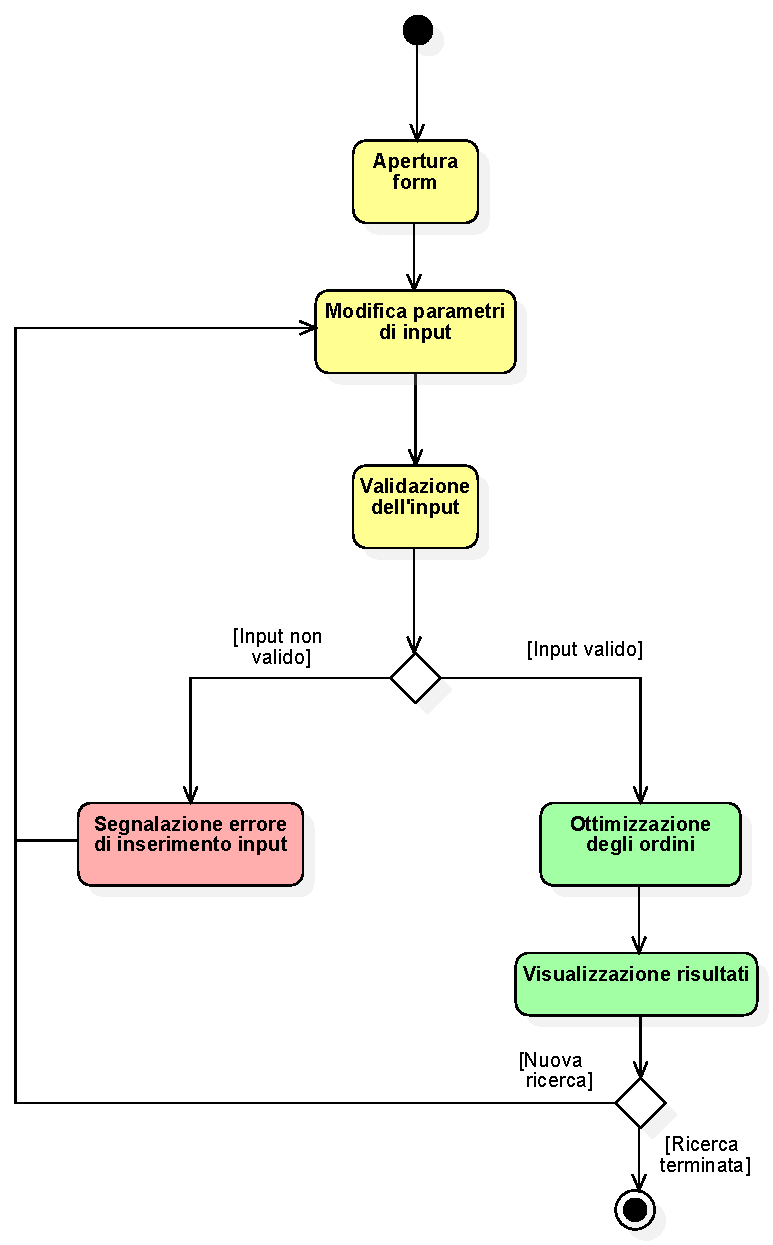
\includegraphics[scale = 0.75]{diagrammi attivita/Diagramma di attivita winform.pdf} 
    \caption{Diagramma di attività della WinForm}
    \label{diagramma-attivita-winform}
\end{figure}

\noindent L'utente, all'apertura della WinForm, modifica i parametri di input che sono:
\begin{itemize}
    \item data di previsione iniziale
    \item data di previsione finale
    \item metodo di risoluzione dei vincoli
\end{itemize}
\noindent Dopo aver scelto gli input, questi vengono validati in modo tale da bloccare anzitempo
l'esecuzione in caso di errori.
Se la validazione va a buon fine allora l'algoritmo calcola la soluzione e vengono visualizzati i risultati.
A questo punto la ricerca può terminare oppure può continuare con la possibilità di variare i parametri di input.

%**************************************************************
\section{Tabu Search}
\label{sec:tabu-search}
\noindent Nella sezione § \ref{conclusione-studio-fattibilita}
riguardante lo studio di fattibilità è emerso come la tabu search
sia il giusto compromesso in termini di efficacia, efficienza
e complessità a livello implementativo.\\
In figura \ref{diagramma-attivita-tabu-search}
viene rappresentato il funzionamento dell'algoritmo ad alto livello.
\vspace*{\fill}
\begin{figure}[!h] 
    \centering 
    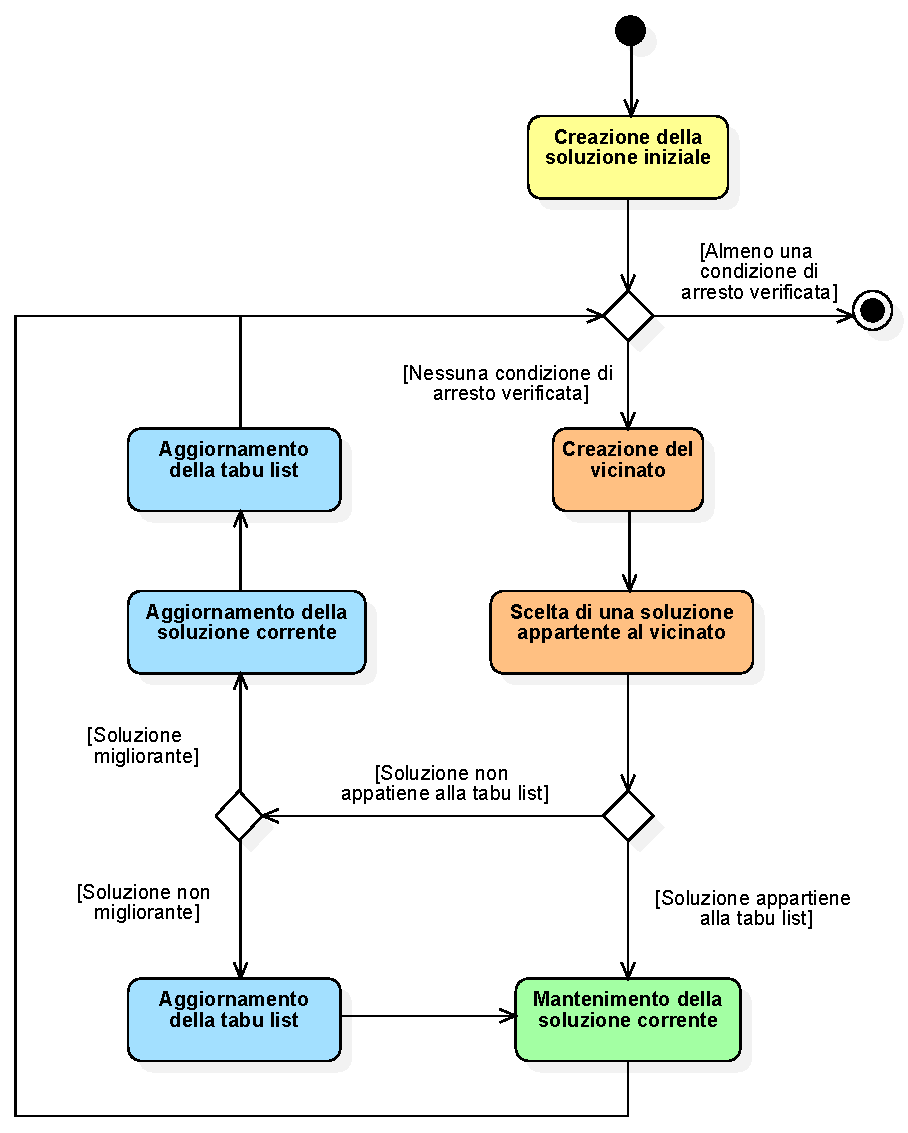
\includegraphics[width=0.8\columnwidth]{diagrammi attivita/diagramma attivita tabusearch.pdf} 
    \caption{Diagramma di attività della tabu search}
    \label{diagramma-attivita-tabu-search}
\end{figure}
\noindent \paragraph{}\hfill\\
Come si può notare, prima viene effettuato un controllo per vedere se la mossa
appartiene o meno alla tabu list e poi viene verificato se la soluzione è migliorante.
Se i controlli venissero invertiti, si rischierebbe, calcolando
la funzione di valutazione e confrontandola con quella della soluzione corrente,
di simulare inutilmente una mossa che potenzialmente potrebbe appartenere alla tabu list.
\vspace*{\fill}

\newpage

%**************************************************************
\subsection{Rappresentazione della soluzione}
\label{sec:rappresentazione-della-soluzione}
\noindent Definire una buona rappresentazione della soluzione è fondamentale
poichè è legata alla creazione del vicinato.\\
In primis è stata creata una classe che rappresentasse
il singolo ordine (dataSourceItem) e, dato che gli ordini solitamente sono molteplici,
si è deciso di mettere ognuno di essi all'interno di una lista.
Questo approccio è sufficiente per un algoritmo greedy, ma non per la tabu search.\\
Infatti è necessario associare alla soluzione anche una funzione di valutazione, in modo tale
da poter operare il confronto tra la soluzione corrente e quella migliore.\\
In figura \ref{rappresentazione-soluzione} viene illustrata la forma della soluzione della tabu search.
\begin{figure}[!h] 
    \centering 
    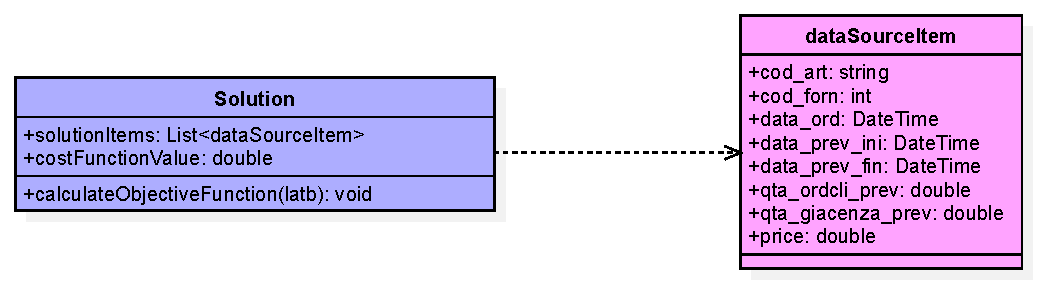
\includegraphics[width=0.8\columnwidth]{soluzione/soluzione rappresentazione.pdf} 
    \caption{Rappresentazione della soluzione per la tabu search}
    \label{rappresentazione-soluzione}
\end{figure}

%**************************************************************
\subsection{Soluzione iniziale}
\label{sec:soluzione-iniziale}
\noindent Nella figura \ref{diagramma-attivita-tabu-search} il primo step è la creazione di una soluzione iniziale che
però la tabu search, a contrario di altri algoritmi, non è in grado di generare da sola. Per ovviare a questo inconveniente
si può generare una soluzione abbastanza buona tramite un algoritmo greedy.\\
Di seguito viene presentato lo pseudocodice.
\vspace*{\fill}
\begin{algorithm}
    \captionsetup{labelformat=empty}
    \caption{Pseudocodice soluzione iniziale - Algoritmo Greedy}
    \vspace{0.1cm}
    \hspace*{\algorithmicindent} \textbf{Input:} {$lista\_articoli$}, {$lista\_spedizioni$}, {$lista\_prezzi$}\\
    \hspace*{\algorithmicindent} \textbf{Output:} {$lista\_articoli\_opt$}
    \begin{algorithmic}[1]
        \Procedure{My\_Greedy\_Algorithm}{$lista\_articoli$, $lista\_spedizioni$, $lista\_prezzi$}
        \State {$l \gets lista\_vuota$}
        \State {$l_{tmp} \gets lista\_vuota$}
        \State $l_{cod\_art} \gets genera\_lista\_decisione(lista\_articoli)$
        \State $n_{cod\_art} \gets l_{cod\_art}.Length$
        \While {$count < n_{cod\_art}$}
            \State {$cod\_art \gets decisione(l_{cod\_art})$}
            \ForAll {$art \in lista\_articoli$}
                \State {$b \gets controllo\_condizioni(art$, $cod\_art$, $lista\_spedizioni$, $lista\_prezzi)$}
                \If {$b = true$}
                    \State Aggiungi $art$ a $l_{tmp}$
                \EndIf
            \EndFor
            \State {$count \gets count+1$}
        \EndWhile
        \State $l \gets filtra\_articoli\_per\_min(l_{tmp})$
        \State \Return $l$
        \EndProcedure
    \end{algorithmic}
\end{algorithm}
\vspace*{\fill}
\newpage
\noindent Si può notare come la funzione $controllo\_condizioni()$ abbia lo scopo di escludere tutte le casistiche relative a tutti i $cod\_art$ in cui:
\begin{itemize}
    \item la data di spedizione è minore del giorno attuale
    \item la data di arrivo della spedizione è maggiore della data di inizio copertura
    \item dato un fornitore, non esiste un prezzo associato ad alcuna spedizione
    \item dato un fornitore, non esiste alcuna spedizione associata ad un prezzo
\end{itemize}

\noindent La funzione $filtra\_articoli\_per\_min()$, avente come parametro di input $l_{tmp}$ (lista con tutti i record che soddisfano i vincoli),
serve invece a filtrare per prezzo minimo tutti i range di copertura associati ad ogni codice articolo.
In pratica per ogni range di copertura di ogni articolo viene preso il record con il fornitore che offre il fabbisogno al prezzo più vantaggioso.\\

\noindent É possibile avere anche un'inizializzazione della soluzione che non sia stata soggetta ad alcuna ottimizzazione.
In questo caso è stata creata una funzione $initialise\_solution()$ che, dati in input gli stessi parametri dell'algoritmo greedy, fornisce
come soluzione iniziale proprio quella generata dal modulo già esistente. 

%**************************************************************
\subsection{Mosse}
\label{sec:mosse}
\noindent Le mosse create per la Tabu Search sono le seguenti:
\begin{enumerate}
    \item Inserimento di un nuovo ordine d'acquisto
    \item Cambio di fornitore di un ordine d'acquisto
    \item Pre-ordine di un ordine d'acquisto
    \item Post-ordine di un ordine d'acquisto
\end{enumerate}
Come si può notare non è stata creata la mossa inversa dell'inserimento, ovvero la rimozione di un ordine d'acquisto.
Il motivo sta nel fatto che rimuovere un ordine di un articolo di cui si ha bisogno non porta sicuramente a un miglioramento
della funzione di valutazione poichè, essendo l'articolo una necessità, prima o poi verrà aggiunto nuovamente.

%**************************************************************
\subsection{Esplorazione del vicinato}
\label{sec:esplorazione-vicinato}
\noindent Il vicinato è quell'insieme di soluzioni che possono essere raggiunte
tramite l'applicazione di una mossa sulla soluzione corrente (chiamata anche centro del vicinato).\\
Si può notare come la dimensione del vicinato in questo problema sia dell'ordine di $O(n!)$ e sia dettata dal fatto che
per ogni range di copertura di ogni articolo sia necessario scegliere la miglior
combinazione tra data d'ordine e fornitore.\\
Data la sua alta complessità non è dunque possibile visitare l'intero vicinato,
motivo per il quale si è deciso di procedere randomizzando le scelte.
In particolare ogni mossa viene selezionata in maniera casuale cosicché tutte le scelte
abbiano la stessa probabilità di essere selezionate.\\
Per lo stesso motivo è stato applicato lo stesso principio anche per la scelta dell'articolo su cui applicare
la mossa.\\
É importante sottolineare come l'oggetto \textit{Random} in C\#
debba essere inizializzato tramite un numero, ovvero
ciò che viene definito come seed. Infatti se non si dichiara
il seed all'interno del costruttore, viene utilizzato il
Current System Time. Questo risultava un problema poichè essendo le
iterazioni molto rapide (a volte anche $<1ms$) si andava ad inizializzare la nuova istanza
di Random allo stesso valore e dunque veniva generato lo stesso
numero, cosa assolutamente indesiderata.


%**************************************************************
\subsection{Tabu List}
\label{sec:tabu-list}
\noindent La tabu list è una lista che memorizza le k mosse precedenti, dove k è uguale
alla lunghezza della lista che viene definita alla creazione dell'oggetto \textit{TabuSearch}.\\
Permette di evitare dunque cicli infiniti in corrispondenza
di minimi locali. Questo accade perché tramite le funzione $generate\_move\_string()$ ogni mossa
viene prima codificata, poi viene effettuata una ricerca nella tabu list, impedendo potenzialmente all’algoritmo di riprovarla,
e infine viene aggiunta nella lista sia nel caso in cui venga effettuata che nel caso in cui non venga effettuata perchè non migliorante.\\
Per semplificare la codifica si salva solamente la stringa generata dalla funzione che rappresenta la mossa e non l’intera
soluzione come previsto dalla teoria.
Si è deciso inoltre di memorizzare, oltre alla mossa eseguita, anche la sua inversa
(per esempio l'inversa del pre-ordine è il post-ordine). Così facendo si
evitano le inversioni immediate che risulterebbero poco sensate e rallenterebbero la ricerca.

%**************************************************************
\subsection{Funzione di valutazione}
\label{sec:funzione-valutazione}
\noindent I parametri da considerare per valutare la bontà di una soluzione, vista dal lato utente,
sono i seguenti:
\begin{itemize}
    \item il numero di articoli ordinati rispetto a quelli totali
    \item il prezzo totale di tutti gli ordini effettuati
\end{itemize}
Chiaramente la funzione di valutazione deve migliorare
se aumenta il numero di articoli ordinati
oppure il prezzo totale diminuisce a parità di articoli ordinati.
Al contrario si ha un peggioramento nel caso in cui a parità di articoli ordinati
corrisponde un prezzo totale maggiore. Non si potrà mai
avere invece un peggioramento della funzione di valutazione causato dalla diminuzione del numero di articoli
ordinati, come spiegato nella sezione §\ref{sec:mosse}.\\
La funzione di valutazione, in questo caso, non può rappresentare perfettamente il
comportamento dell'algoritmo e definisce dunque un'approssimazione del suo andamento.\\
Durante la ricerca sono state provate empiricamente 3 funzioni che vengono elencate qui sotto:
\vspace{1cm}
\begin{center}
    \begin{minipage}{.5\textwidth}
        \begin{itemize}
            \item[] \text{\large $f = \frac{PT \cdot (1-R)}{e^{R}}$}
            \item[] \text{\large $g=\begin{cases} \frac{ln(PT) \cdot (1-R)}{e^{R}} & \mbox{se }R\neq 1 \\ -\frac{1}{PT} & \mbox{se }R=1\end{cases}$}
            \item[] \text{\large $h=\begin{cases} \frac{ln(PT+1) \cdot (1-R)}{e^{R}} & \mbox{se }R\neq 1 \\ -\frac{1}{PT} & \mbox{se }R=1\end{cases}$}
        \end{itemize}
    \end{minipage}
\end{center}
\vspace*{1cm}
\noindent dove:
\begin{itemize}
    \item $PT = $ Prezzo totale
    \item $OE = $ numero di articoli ordinati
    \item $OT = $ numero di articoli da ordinare
    \item $R =$ \text{\large $\frac{OE}{OT}$} $=$ rapporto tra gli articoli ordinati e quelli da ordinare
\end{itemize}

\newpage

\noindent Nelle tabelle \ref{tab:risultati-f}, \ref{tab:risultati-g} e \ref{tab:risultati-h} vengono riportati i risultati che sono stati calcolati
per capire empiricamente quale fosse la funzione di valutazione
che approssimasse meglio il comportamento dell'algoritmo.\\

\begin{table}[!h]
    \begin{minipage}{.5\linewidth}
        \caption{Tabella dei risultati di $f$}
        \label{tab:risultati-f}
        \rowcolors{2}{lightest-grayest}{white}
        \begin{tabular}{|c|c|c|c|}
        \hline
        \rowcolor{lighter-grayer}
        \centering \textbf{PT} & \multicolumn{2}{c}{\centering \textbf{Rapporto $\frac{OE}{OT}$}} & \centering \textbf{FV} \arraybackslash \\
        \hline
        
        \fval{250.000}{30}{0,0230}{238.659,21}
        \fval{400.000}{40}{0,0307}{375.944,97}
        \fval{500.000}{50}{0,0384}{462.629,19}
        \fval{600.000}{60}{0,0461}{546.493,78}
        \fval{350.000}{21}{0,0161}{338.828,33}
        \fval{350.000}{22}{0,0169}{338.303,08}
        \fval{350.000}{23}{0,0176}{337.778,43}
        \fval{400.000}{23}{0,0176}{386.032,50}
        \fval{400.000}{24}{0,0184}{385.433,60}
        \fval{500.000}{1300}{1,0000}{0,00000000}
        \fval{450.000}{1300}{1,0000}{0,00000000}
        \end{tabular}
    \end{minipage}
    \begin{minipage}{.5\linewidth}
        \caption{Tabella dei risultati di $g$ }
        \label{tab:risultati-g}
        \rowcolors{2}{lightest-grayest}{white}
        \begin{tabular}{|c|c|c|c|}
        \hline
        \rowcolor{lighter-grayer}
        \centering \textbf{PT} & \multicolumn{2}{c}{\centering \textbf{Rapporto $\frac{OE}{OT}$}} & \centering \textbf{FV} \arraybackslash \\
        \hline
        \fval{250.000}{30}{0,0230}{11,8653876}
        \fval{400.000}{40}{0,0307}{12,1234920}
        \fval{500.000}{50}{0,0384}{12,1415767}
        \fval{600.000}{60}{0,0461}{12,1182126}
        \fval{350.000}{22}{0,0169}{12,3390619}
        \fval{350.000}{23}{0,0176}{12,3199264}
        \fval{400.000}{23}{0,0176}{12,4487951}
        \fval{400.000}{24}{0,0184}{12,4294818}
        \fval{0,75}{1}{0,0008}{-0,2872397}
        \fval{500.000}{1300}{1,0000}{-0,0000020}
        \fval{450.000}{1300}{1,0000}{-0,0000022}
        \end{tabular}
    \end{minipage}
\end{table}


\begin{table}[!h]
    \centering
    \caption{Tabella dei risultati di $h$}
    \label{tab:risultati-h}
    \rowcolors{2}{lightest-grayest}{white}
    \begin{tabular}{|c|c|c|c|}
    \hline
    \rowcolor{lighter-grayer}
    \centering \textbf{PT} & \multicolumn{2}{c}{\centering \textbf{Rapporto $\frac{OE}{OT}$}} & \centering \textbf{FV} \arraybackslash \\
    \hline
    \fval{250.000}{30}{0,0230}{11,8653914}
    \fval{400.000}{40}{0,0307}{12,1234943}
    \fval{500.000}{50}{0,0384}{12,1415785}
    \fval{600.000}{60}{0,0461}{12,1182141}
    \fval{350.000}{22}{0,0169}{12,3390647}
    \fval{350.000}{23}{0,0176}{12,3199292}
    \fval{400.000}{23}{0,0176}{12,4487975}
    \fval{400.000}{24}{0,0184}{12,4294842}
    \fval{0,75}{1}{0,0008}{0,55875534}
    \fval{500.000}{1300}{1,0000}{-0,0000020}
    \fval{450.000}{1300}{1,0000}{-0,0000022}
    \end{tabular}
\end{table}

\noindent É evidente dalla tabella \ref{tab:risultati-f}
come la funzione $f$ sia migliorativa se il prezzo totale
degli ordini è minore, ma non lo sia nel caso
di aumento del numero di articoli ordinati. Questo problema accade
perchè il rapporto tra $R$ e $PT$ è troppo sbilanciato.\\
Altra problematica è il fatto che la funzione, una volta ordinati
tutti gli articoli, non riesce a valutare la variabile $PT$
in quanto $1-R$ è uguale a $0$.\\
Si è optato quindi per la modifica della funzione di valutazione
e si è ottenuta la funzione $g$.\\

\noindent Si osservi ora la tabella \ref{tab:risultati-g}.
Per cercare di risolvere il primo problema, si è deciso di
adottare un compromesso andando ad utilizzare il logaritmo naturale.\\
Dal quinto all'ottavo risultato si può evincere che:
\begin{enumerate}
    \item a parità di $PT$ $\rightarrow$ $FV$ è migliore per
    un $R$ minore
    \item a parità di $R$ $\rightarrow$ $FV$ è migliore per
    un $PT$ minore
\end{enumerate}
Tuttavia si può notare come non sia stato comunque completamente
risolto il problema perchè nei primi tre risultati
$FV$ aumenta e solo nel quarto inizia a decrescere.
Questo potrebbe sembrare un problema, ma in realtà non lo è in
quanto la mossa disponibile nella tabu search inserisce
un elemento per volta riconducendoci quindi
più verosimilmente alle casistiche dell'intervallo che va dal quinto all'ottavo risultato.\\

\noindent Per il secondo problema invece si è dovuto procedere per casi in
base al valore assunto da $R$. In questo modo, non appena
tutti gli articoli sono stati ordinati ($R=1$), è possibile operare
un confronto.
Data dunque $FV$ definita come il negativo del reciproco di $R$,
è facile vedere come al diminuire di $R$ diminuisce anche $FV$
risolvendo dunque completamente il problema.\\\\

\noindent Il decimo risultato è stato determinante poichè ha permesso di
scoprire un altro problema che è principalmente di dominio.
Infatti la funzione $g$ valuta tutte i risultati con $0 < PT < 1$
e $R<1$ come miglioranti persino rispetto a quei
risultati con $R=1$. Per risolvere questo problema si è andati
a rimodificare la funzione di valutazione ottenendo $h$.\\

\noindent Si osservi ora la tabella \ref{tab:risultati-h}.
Per risolvere il problema esposto precedentemente si è andato
a modificare il dominio della funzione aggiungendo una unità.
In questo modo per ogni valore di $PT$ si avrà che
$ln(PT+1)>0$ facendo in modo che $FV$ sia negativa se e solo se
$R=1$.

%**************************************************************
\subsection{Condizioni di arresto}
\label{sec:condizioni-arresto}
\noindent La Tabu Search si ferma se si verifica almeno una delle seguenti condizioni:
\begin{itemize}
    \item \textbf{Numero massimo di iterazioni:} numero di mosse eseguibili dall'algoritmo, deciso
    dal programmatore, che permette di evitare la possibilità di eventuali cicli infiniti;
    \item \textbf{Numero massimo di iterazioni non migliorative:} numero di mosse non migliorative
    consecutive eseguibili dall'algoritmo, deciso dal programmatore, che permette
    di rilevare in maniera approssimativa un minimo
    locale e terminare la procedura;
    \item \textbf{Tempo massimo di esecuzione:}  durata temporale oltre
    la quale il programma si ferma automaticamente. Questo serve per venire incontro a
    bisogni di rapidità di risposta da parte dell’azienda.
    
\end{itemize}
%**************************************************************
\subsection{Controllo dei vincoli}
\label{sec:controllo-vincoli}
\noindent Nel programma i vincoli vengono sempre controllati alla fine dell'esecuzione dell'algoritmo
tramite due funzioni:
\begin{itemize}
    \item $control\_Min\_Order\_Articles()$, con input la
    lista di ordini effettuati e la lista dei bound rispetto
    al singolo ordine
    \item $control\_Mins\_Forn()$, con input la lista di
    ordini effettuati, la lista delle date di spedizione,
    la lista dei bound dei fornitori e la scelta della
    modalità di risoluzione dei vincoli
\end{itemize}
\newpage
\noindent La prima funzione controlla per ogni range di
copertura di ogni articolo che l'ordine:
\begin{enumerate}
    \item rispetti il quantitativo minimo
    da ordinare in quella specifica data d'ordine;
    \item venga effettuato per multipli se il quantità
    dell'ordine supera il quantitativo minimo da ordinare
\end{enumerate}
Il primo vincolo viene risolto aggiungendo la differenza alla quantità attuale
in modo tale da arrivare al minimo.
Il secondo viene risolto in questo modo:
\begin{enumerate}
    \item si trova la differenza tra la quantità attuale
    e quella minima richiesta
    \item viene eseguito il modulo tra la differenza calcolata al punto 1 e il valore del multiplo
    \item viene aggiunta alla quantità attuale la differenza tra il valore del multiplo e il valore calcolato al punto precedente 
\end{enumerate}
\vspace*{0.5cm}
\noindent La seconda funzione, invece, controlla per ogni 
periodo e per ogni fornitore a cui si abbia fatto
almeno un ordine che:
\begin{itemize}
    \item il numero degli articoli totali comprati all'interno
    del determinato periodo sia maggiore del bound
    \item l'importo totale all'interno del periodo sia
    maggiore del bound
\end{itemize}
Per la soddisfazione di questi due vincoli, l'utente ha la
possibilità di scegliere quale tra le seguenti tecniche adottare:
\begin{enumerate}
    \item \textbf{Min/Max:} per il primo (risp. secondo) vincolo
    consiste nel scegliere l'articolo minimo (risp. massimo)
    da aumentare e appartente al periodo per arrivare al
    minimo dichiarato dal bound
    \item \textbf{Proporzionale:} consiste nel continuare a ciclare
    tutti gli articoli appartenti al periodo e aumentarli di
    una unità finchè non si è raggiunto il minimo
    dichiarato dal bound.
    \item \textbf{Ricompattamento:} consiste nel selezionare l'ordine
    successivo con lo stesso fornitore, con il prezzo minimo e
    non appartenente al periodo in modo tale anticipare l'acquisto
    e non ordinare articoli in più.
\end{enumerate}
\vspace*{0.5cm}
\noindent Questi controlli vengono effettuati solo alla fine dall'algoritmo.
Questo implica che la tabu search può potenzialmente avere in
una qualsiasi iterazione una soluzione non ammissibile e
continuare ad operare con essa. Tuttavia poichè alla fine
l'algoritmo restituisce una soluzione ottima, che corrisponde
alla miglior combinazione per ogni range di copertura di
ogni articolo tra data d'ordine e fornitore, l'ottimo non viene
influenzato, ma vincolato.\\
Inoltre se si volessero fare i controlli durante l'esecuzione dell'algoritmo,
oltre a rallentarlo notevolmente, si avrebbe un importante aumento di
complessità in quanto sarebbe necessario salvare le quantità realmente
necessarie in un'altra lista e operare altri controlli.

\newpage

%**************************************************************
\section{Codifica}
\label{sec:codifica}
\noindent In questa sezione verranno trattate le parti principali e più interessanti riguardo l'attività
di codifica e realizzazione dell'algoritmo.

%**************************************************************
\subsection{Organizzazione dello sviluppo}
\label{sec:organizzazione-sviluppo}
\noindent Il servizio e le sue funzionalità sono state sviluppate in un
ordine preciso. Si è cercato di implementare il prodotto
con un approccio incrementale, in modo tale da avere
sempre un prodotto funzionante.\\
In particolare, lo sviluppo è stato svolto nel seguente ordine:
\begin{itemize}
    \item creazione della winform
    \item lettura dei dati dal database
    \item pre-processing dei dati
    \item costruzione dell'algoritmo greedy
    \item costruzione di altre scelte greedy
    \item costruzione della tabu search
    \item lettura dei vincoli
    \item costruzione dei vari metodi risolutivi
    per il soddisfacimento dei vincoli
\end{itemize}

\noindent Quest'ordine ha permesso di concentrarsi su obiettivi specifici,
facilitandone dunque l'implementazione sia a livello logico che a livello pratico.\\

\noindent Al raggiungimento di ogni \textit{milestone} veniva
organizzata un brevissima discussione con il tutor
in cui veniva verificata la correttezza e la coerenza di quanto
sviluppato in relazione agli obiettivi preposti.
%**************************************************************
\subsection{Log}
\label{sec:log}
\noindent Su richiesta di Ergon Informatica è stato aggiunto successivamente il requisito \hyperref[tab:requisiti-qualitativi]{R40-Q-D}
riguardante lo svolgimento da parte del programma di attività di scrittura
su file. Ad ogni avvio della tabu search viene creato un nuovo
file denominato come \textit{"Log\_aaaa\_mm\_gg\_hh\_mm\_ss"}
dove vengono salvati dati ad ogni iterazione, quali:
\begin{itemize}
    \item l'iterazione corrente
    \item cosa è accaduto all'interno dell'iterazione (mossa tabu, non migliorante, effettuata)
    \item il numero di iterazioni non miglioranti
    \item il tempo di esecuzione corrente
    \item valore della funzione di valutazione della migliore soluzione corrente
\end{itemize}
Il salvataggio di queste informazioni ha
l’obiettivo di facilitare il debug
del codice e la rilevazione dei dati ottenuti
dall’algoritmo ad ogni iterazione.\\
Inoltre questi dati possono essere utilizzati anche in futuro
per operare confronti fra esecuzioni della tabu search con
tipologie di inizializzazione differenti.

\newpage

%**************************************************************
\subsection{Estensioni del progetto}
\label{sec:estensioni-progetto}
\noindent Alla fine del percorso di stage è stato richiesto di
elencare eventuali feature ed estensioni che si possono
applicare al progetto.
\vspace*{0.3cm}
\noindent \paragraph{Nuovo algoritmo}\hfill\\
La creazione della tabu search e dell'algoritmo greedy non esclude
lo sviluppo di un nuovo algoritmo. Infatti grazie all'utilizzo del design
pattern \textit{strategy} è possibile estendere l'interfaccia
\textit{AlgorithmStrategy} e nella classe \textit{Program}
creare il corrispondente oggetto del nuovo algoritmo.
Chiaramente, affinchè la classe sia istanziabile, è necessario
implementare tutte le funzioni dell'interfaccia.\\
Si potrebbe valutare, in base alle risorse a disposizione, la creazione di un algoritmo genetico oppure di una combinazione tra la tabu search e un altro algoritmo
e provare a mettere i risultati a confronto.
\vspace*{0.3cm}
\noindent \paragraph{Nuova scelta greedy}\hfill\\
Le scelte greedy esistenti sono utilizzate per andare
a creare degli algoritmi che forniscono buone soluzioni.
Tuttavia possono esistere delle scelte che non sono state ancora
considerate e che portino alla creazione di un algoritmo
che genera soluzioni migliori.\\
Grazie all'utilizzo del design pattern strategy è possibile estendere
la classe astratta \textit{GreedyAlgorithm}, quest'ultima derivante dall'interfaccia
\textit{AlgorithmStrategy}.\\
Una possibile scelta potrebbe essere quella di selezionare
l'articolo più economico del fornitore che ha più richieste d'ordine
oppure l'articolo più richiesto del fornitore
che ha la minor media delle variazioni dei suoi articoli.
\vspace*{0.3cm}
\noindent \paragraph{Nuova mossa della tabu search}\hfill\\
Le mosse attuali della tabu search sono semplici e rapide,
creando una bassa perturbazione della miglior soluzione
(o centro del vicinato). Tuttavia potrebbe essere necessaria
una qualche mossa più complessa in modo tale da visitare
più velocemente lo spazio delle soluzioni.\\
Per esempio si potrebbe pensare di aumentare la molteplicità
di applicazione della mossa.\\ Per esempio se precedentemente
la mossa veniva applicata a un solo codice articolo, si potrebbe
pensare di applicarla a $k$ codici articolo, con $k$
deciso dal programmatore. Rimane comunque fondamentale mantenere
la randomicità delle scelte.
\vspace*{0.3cm}
\noindent \paragraph{Multi-threading}\hfill\\
Questa estensione del progetto andrebbe a considerare la
creazione di più tabu search e di farle eseguire su più thread.
L'idea si basa sul fatto che ogni tabu search viene inizializzata
con una diversa soluzione iniziale in modo tale da diversificare
la ricerca e intensificarla durante l'esecuzione dell'algoritmo
vero e proprio. Ciò potrebbe essere paragonabile alla popolazione
dell'algoritmo genetico dove però non viene effettuata alcuna
ricombinazione, ma ogni soluzione viene trattata singolarmente.
Dopo che tutti i thread hanno terminato l'esecuzione si andrà
a scegliere la soluzione con la funzione di valutazione minore.

\newpage

%**************************************************************
\section{Tecnologie e strumenti}
\label{sec:tecnologie-strumenti}

\noindent Di seguito viene esposta una panoramica delle tecnologie e degli strumenti utilizzati.
Sono stati tutti imposti da Ergon Informatica in quanto sono le tecnologie e gli strumenti
da loro impiegati per lo sviluppo software.\\
Per l’azienda le caratteristiche determinanti della scelta di queste tecnologie
sono riconducibili alle soddisfazione delle seguenti necessità e aspettative:
\begin{itemize}
    \item compatibilità con il sistema Ergdis;
    \item facilità di apprendimento;
    \item ampia disponibilità della documentazione;
    \item gradevolezza dell’interfaccia grafica.
\end{itemize}
Di seguito vegono presentate le tecnologie utilizzate.


\subsection*{C\#}
\begin{figure}[!h] 
    \centering 
    
\includegraphics[scale = 0.04]{loghi/CSharpLogo.pdf} 
    \caption{Logo C\#}
 \end{figure}
\noindent C\# è un linguaggio di programmazione multi-paradigma orientato agli oggetti
sviluppato da Microsoft. La sua sintassi e struttura derivano da altri linguaggi nati
precedentemente, come C++, Java e Visual Basic.\\
C\# è progettato per essere compatibile con le classi e l’ambiente di compilazione
del framework .NET. Supporta astrazione, ereditarietà e polimorfismo
fornendo estensibilità e riusabilità del codice.
È stato ufficialmente approvato come standard dalla ECMA.\\
L'azienda, sebbene abbia sviluppato la maggior parte dei moduli
in Visual Basic, sta lentamente traducendo tutto in questo linguaggio.

\subsection*{Visual Studio 2019}
\begin{figure}[!h] 
    \centering 
    
\includegraphics[scale = 0.75]{loghi/VisualStudio2019Logo.pdf} 
    \caption{Logo Visual Studio 2019}
 \end{figure}
\noindent Visual Studio 2019 è un ambiente di sviluppo integrato (IDE) fornito da Microsoft.
Permette lo sviluppo di software per computer, siti web, applicazioni web, servizi web
e applicazioni mobile. È compatibile con tutte le piattaforme di sviluppo
software Microsoft, quali Windows API e Windows Form.\\
Visual Studio 2019 supporta il refactoring del codice e intellisense, uno strumento per
l’autocompletamento del codice. Il debugger integrato funziona sia a
livello di codice sorgente che a livello di codice macchina. È compatibile anche con i sistemi di supporto per il controllo del codice,
come per esempio Subversion e Git.\\
Visual Studio 2019 supporta 36 differenti linguaggi di 
programmazione tra i quali C\#.

\subsection*{DevExpress}
\begin{figure}[!h] 
    \centering 
    
\includegraphics[scale = 0.35]{loghi/DevExpressLogo.png}
    \caption{Logo DevExpress}
\end{figure}
\noindent DevExpress è una compagnia che produce strumenti di sviluppo software per
Visual Studio. In particolare crea estensioni che vengono utilizzate tramite Visual
Studio per velocizzare la scrittura di applicazioni. Gli strumenti da loro forniti sono
molteplici, in particolare hanno sviluppato controlli .NET di interfaccia utente (UI).
Questi ultimi rendono più semplice la creazione di ambienti grafici per applicazioni ed
elegante il risultato.

\subsection*{Informix}
\begin{figure}[!h] 
    \centering 
    
\includegraphics[scale = 0.04]{loghi/InformixLogo.pdf}
    \caption{Logo IBM Informix}
\end{figure}
\noindent IBM Informix è un prodotto di IBM. La base di dati Informix è usata in molte
applicazioni OLTP ad alto tasso di transazione che operano in vari settori tra cui anche quelli della produzione e dei trasporti.\\
L’Informix server supporta il modello relazionale ad oggetti che permette ad IBM di
offrire estensioni che permettono di effettuare interrogazioni per un dominio specifico
e archiviazioni per set di dati in maniera rapida ed efficiente.
É in grado di supportare sia SQL che NoSQL.

\subsection*{Git}
\begin{figure}[!h] 
    \centering 
    
\includegraphics[scale = 0.4]{loghi/GitLogo.pdf}
    \caption{Logo Git}
\end{figure}
\noindent Git è uno strumento per il controllo di versione distribuito del codice sorgente delle repository.\\
Creato inizialmente per gestire le versioni del kernel Linux, al giorno d'oggi è uno dei principali
strumenti di versionamento del codice e di collaborazione tra gli sviluppatori.